\section{Software Architecture Document}
\label{sec:Software Architecture Document}
% 
% \subsection{Architektonische Repr\"asentation}
% 
% 
% \subsection{Architektonische Faktoren}
% 
% 
\subsection{Architektonische Entscheidungen}
\begin{itemize}
  \item Zu Projektbeginn wurde relativ bald eine Drei-Schichten-Architektur entworfen.
  \item In der Woche 45 wurde entschieden, das Projekt als Maven-Projekt zu halten. Der Entscheid wurde vorallem getroffen, da Properties zentral verwaltet und Tests sauber vom restlichen Sourcecode getrennt gehalten werden k\"onnen.
\end{itemize}
% 
\subsection{Logical View}
\begin{figure}[H]
    \centering
    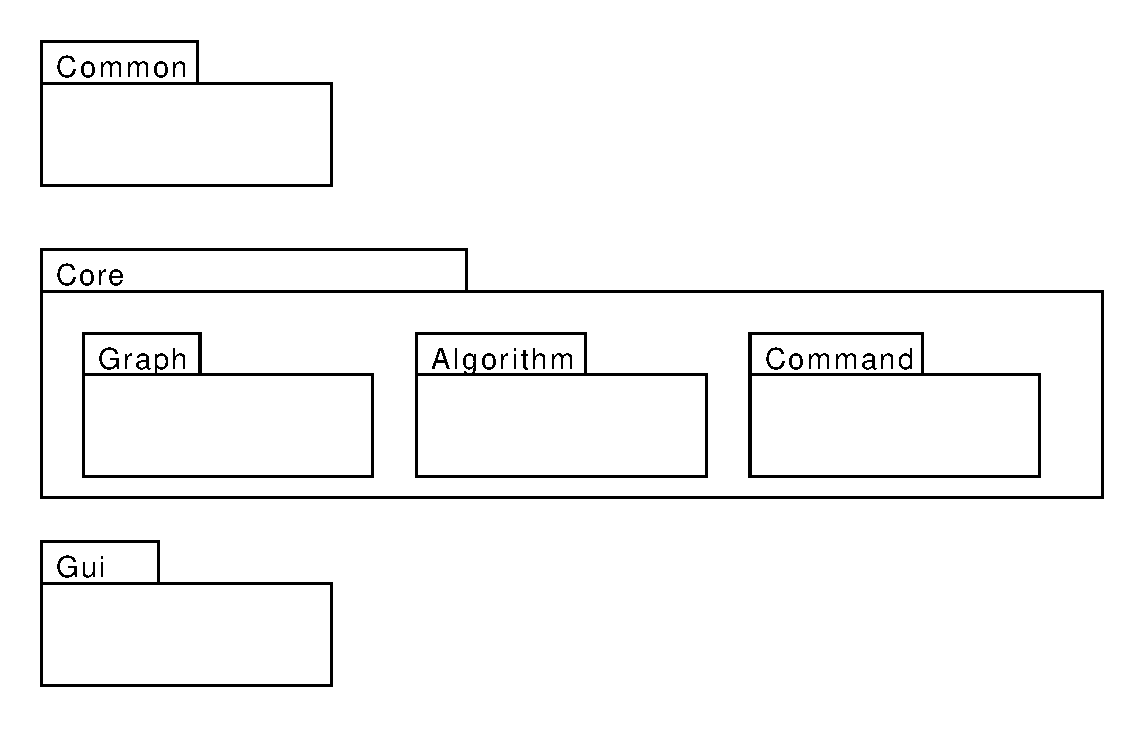
\includegraphics[scale=0.5]{diagrams/package-diagram.pdf}
    \caption{Software Architecture, Package Diagram}
    \label{fig:package-diagram}
\end{figure}
\subsubsection{Beschreibung und Motivation}
Die Systemkomponenten sind in Schichten unterteilt, wobei nur eine h\"oher liegende Schicht direkten Zugriff auf eine darunterliegende Schicht hat (Schichtenarchitektur). F\"ur die Architektur lassen sich von (unten nach oben) grob die Systemkomponenten \textit{Common}, \textit{Core} und \textit{Gui} identifizieren. Die Drei-Schichten-Architektur hat sich aus den Requirements ergeben. Die Komponente Common h\"alt die Interfaces f\"ur einen Actor 'Algorithm Developer' (offstage) bereit, die Komponente Gui enth\"alt die (grafische) Benutzerschnittstelle und schliesslich die Komponente Core: das Herzst\"uck des Systems k\"ummert sich um das Initialisieren der Komponenten, I/O, Verwaltung der Parameter sowie der Berechnung der Traversierung.
% 
% \subsection{Deployment View}
% 
% 
\subsection{Process View}
% 
\subsubsection{Common}
\label{subsubsec:Common}
Die Komponente h\"alt die f\"ur die Implementation eines Algorithmus zu verwendende Schnittstellen bereit. Diese sind f\"ur Algorithmen zu verwenden, welche importiert werden wollen.
% 
\subsubsection{Core}
\label{subsubsec:Core}
Die Komponente implementiert:
\begin{itemize}
  \item Data Model: Datenhaltung f\"ur Graph (Datenelemente Knoten und Kanten), Algorithmus und berechnete Traversierung, Traversierungsschritte als Resultat der Operation eines Algorithmus auf einen Graphen
  \item Business Logik: 
  \begin{itemize}
      \item Handling von Daten-Import und L\"oschen von Daten
      \item Validierung Graphen und Algorithmen beim Import
      \item Handling von Graphen und Algorithmen
      \item Traversierung und damit Erstellen der visualisierbaren L\"osung
  \end{itemize}
  \item Core Inteface: eine Schnittstelle, welche der Komponente GUI zur Verf\"ugung steht
\end{itemize}
% 
\subsubsection{Gui}
\label{subsubsec:Gui}
Die Komponente implementiert ein Model-View-Control (MVC) unter Verwendung des Java-Observer-Pattern:
\begin{itemize}
  \item Model: Observable mit s\"amtlichen GUI-Attributen und deren Getter- und Setter-Methoden
  \item View: Observer mit grafischen Elementen wie z.B. Menubar, Kn\"opfe, Regler und Text-Panelen
  \item Control: Implementiert Listeners und deren Methoden
\end{itemize}
% 
\begin{figure}[H]
    \centering
    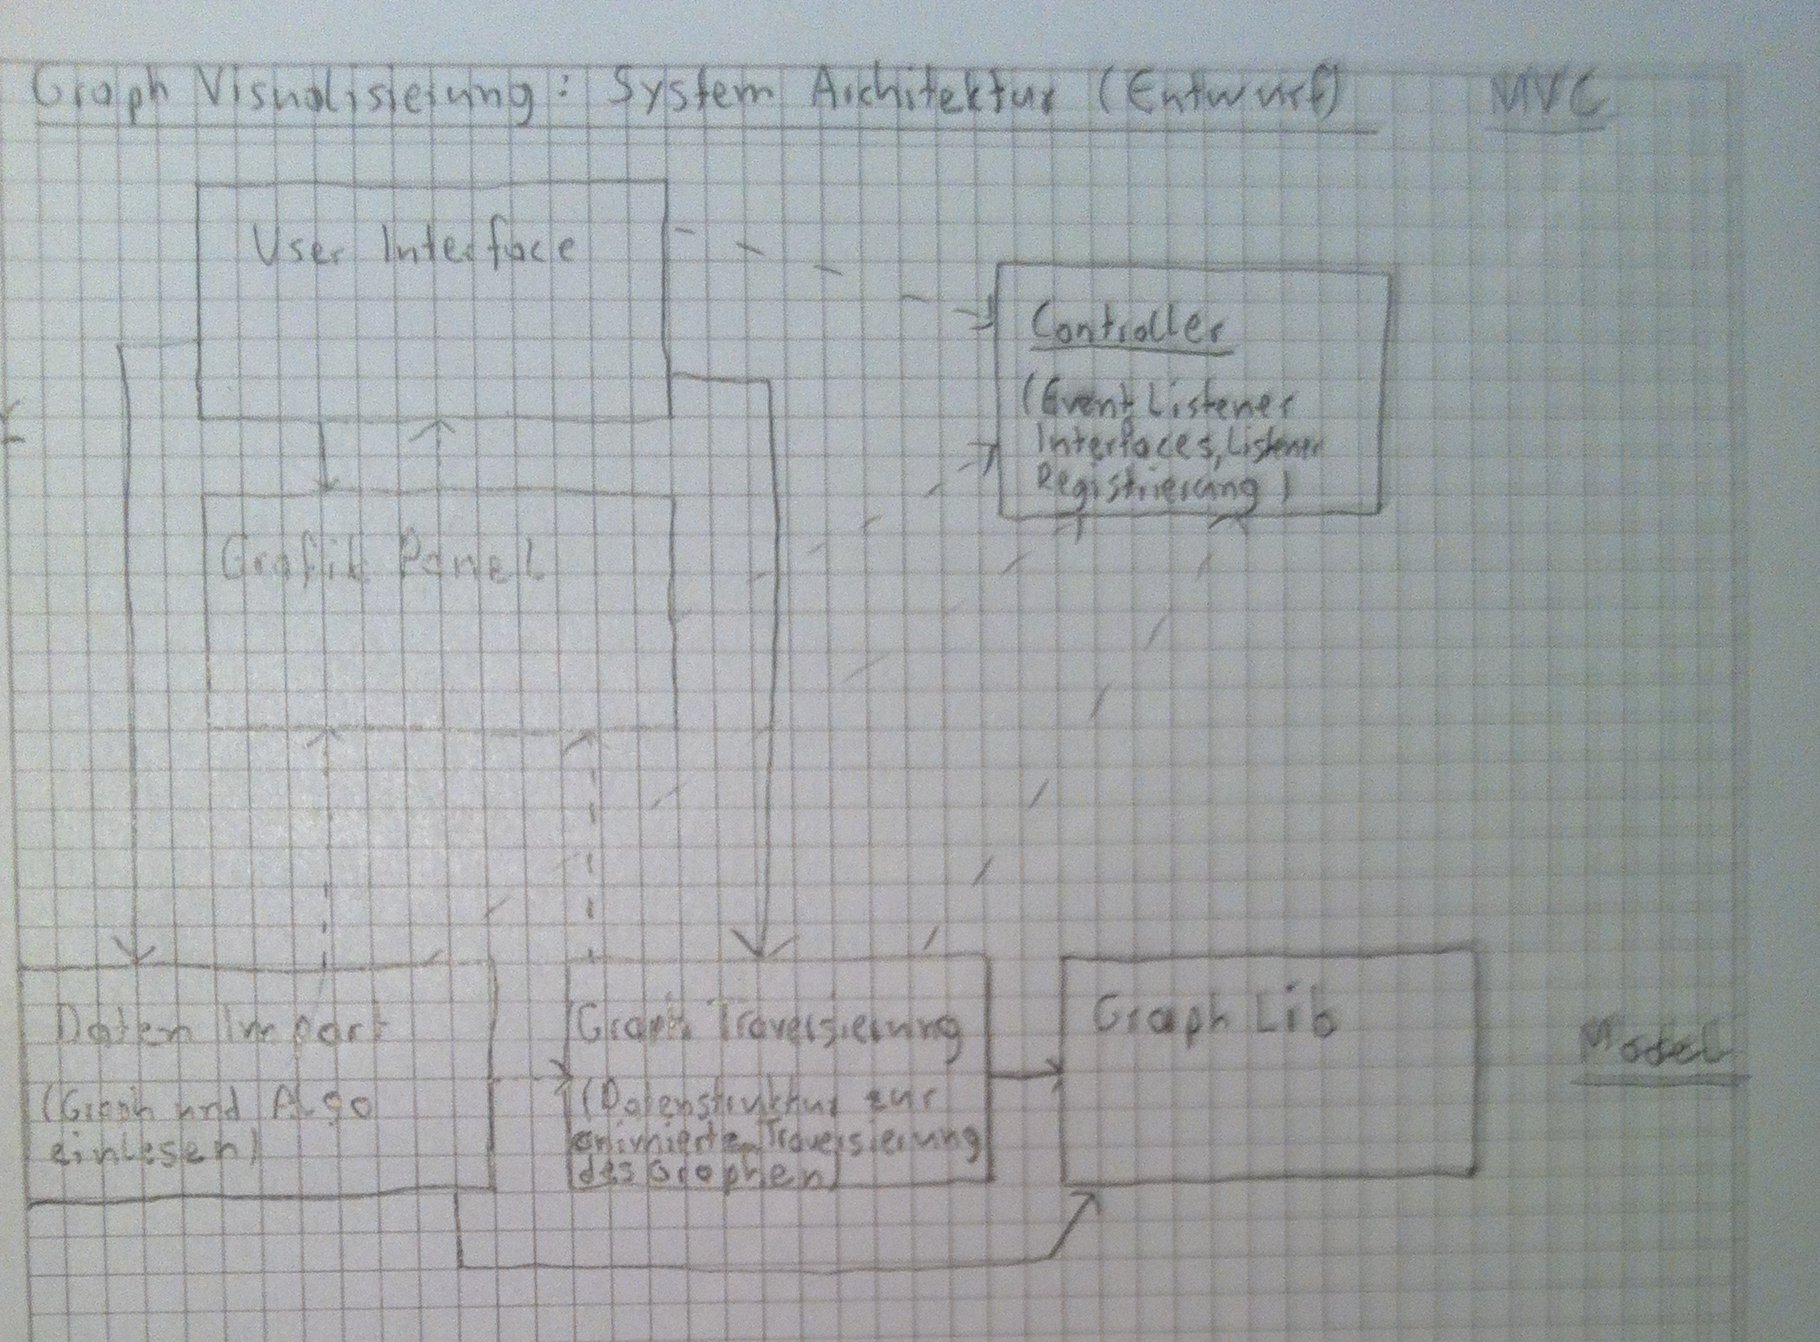
\includegraphics[
% 		    width=\textwidth,
% 		    height=\textheight,
% 		    angle=90,
		    scale=0.1,
		    keepaspectratio=true
    ]{diagrams/architecture/Draft_System_Architecture_PK_V1_cropped.jpeg}
    \caption{Gui, MVC: Conceptual Class Diagram}
    \label{fig:gui-mvc-ccd}
\end{figure}
% 
\subsection{Use-Case View}
Folgende Use Cases wurden implementiert:
\begin{itemize}
  \item Daten:
  \begin{itemize}
    \item Neuen Graphen oder Algorithmus importieren
    \item Importierter Graph oder Algorithmus l\"oschen
  \end{itemize}
  \item Traversierung:
  \begin{itemize}
    \item Graph ausw\"ahlen
    \item Algorithmus ausw\"ahlen
%     \item evt. Start- resp. Endknoten ausw\"ahlen
  \end{itemize}
  \item Visualisierung:
  \begin{itemize}
      \item Einstellen Steplength: Anzahl Traversierungs-Schritte pro Bild
      \item Einstellen Delay: Zeitintervall zwischen zwei Bildern (in Sekunden)      
      \item Visualisierung, Step-by-Step: Ein Bild vor, ein Bild zur\"uck, an das Ende oder den an den Anfang springen
      \item Visualisierung, Animation: Starten, Anhalten, Stoppen
  \end{itemize}
\end{itemize}
% 
\begin{figure}[H]
    \centering
    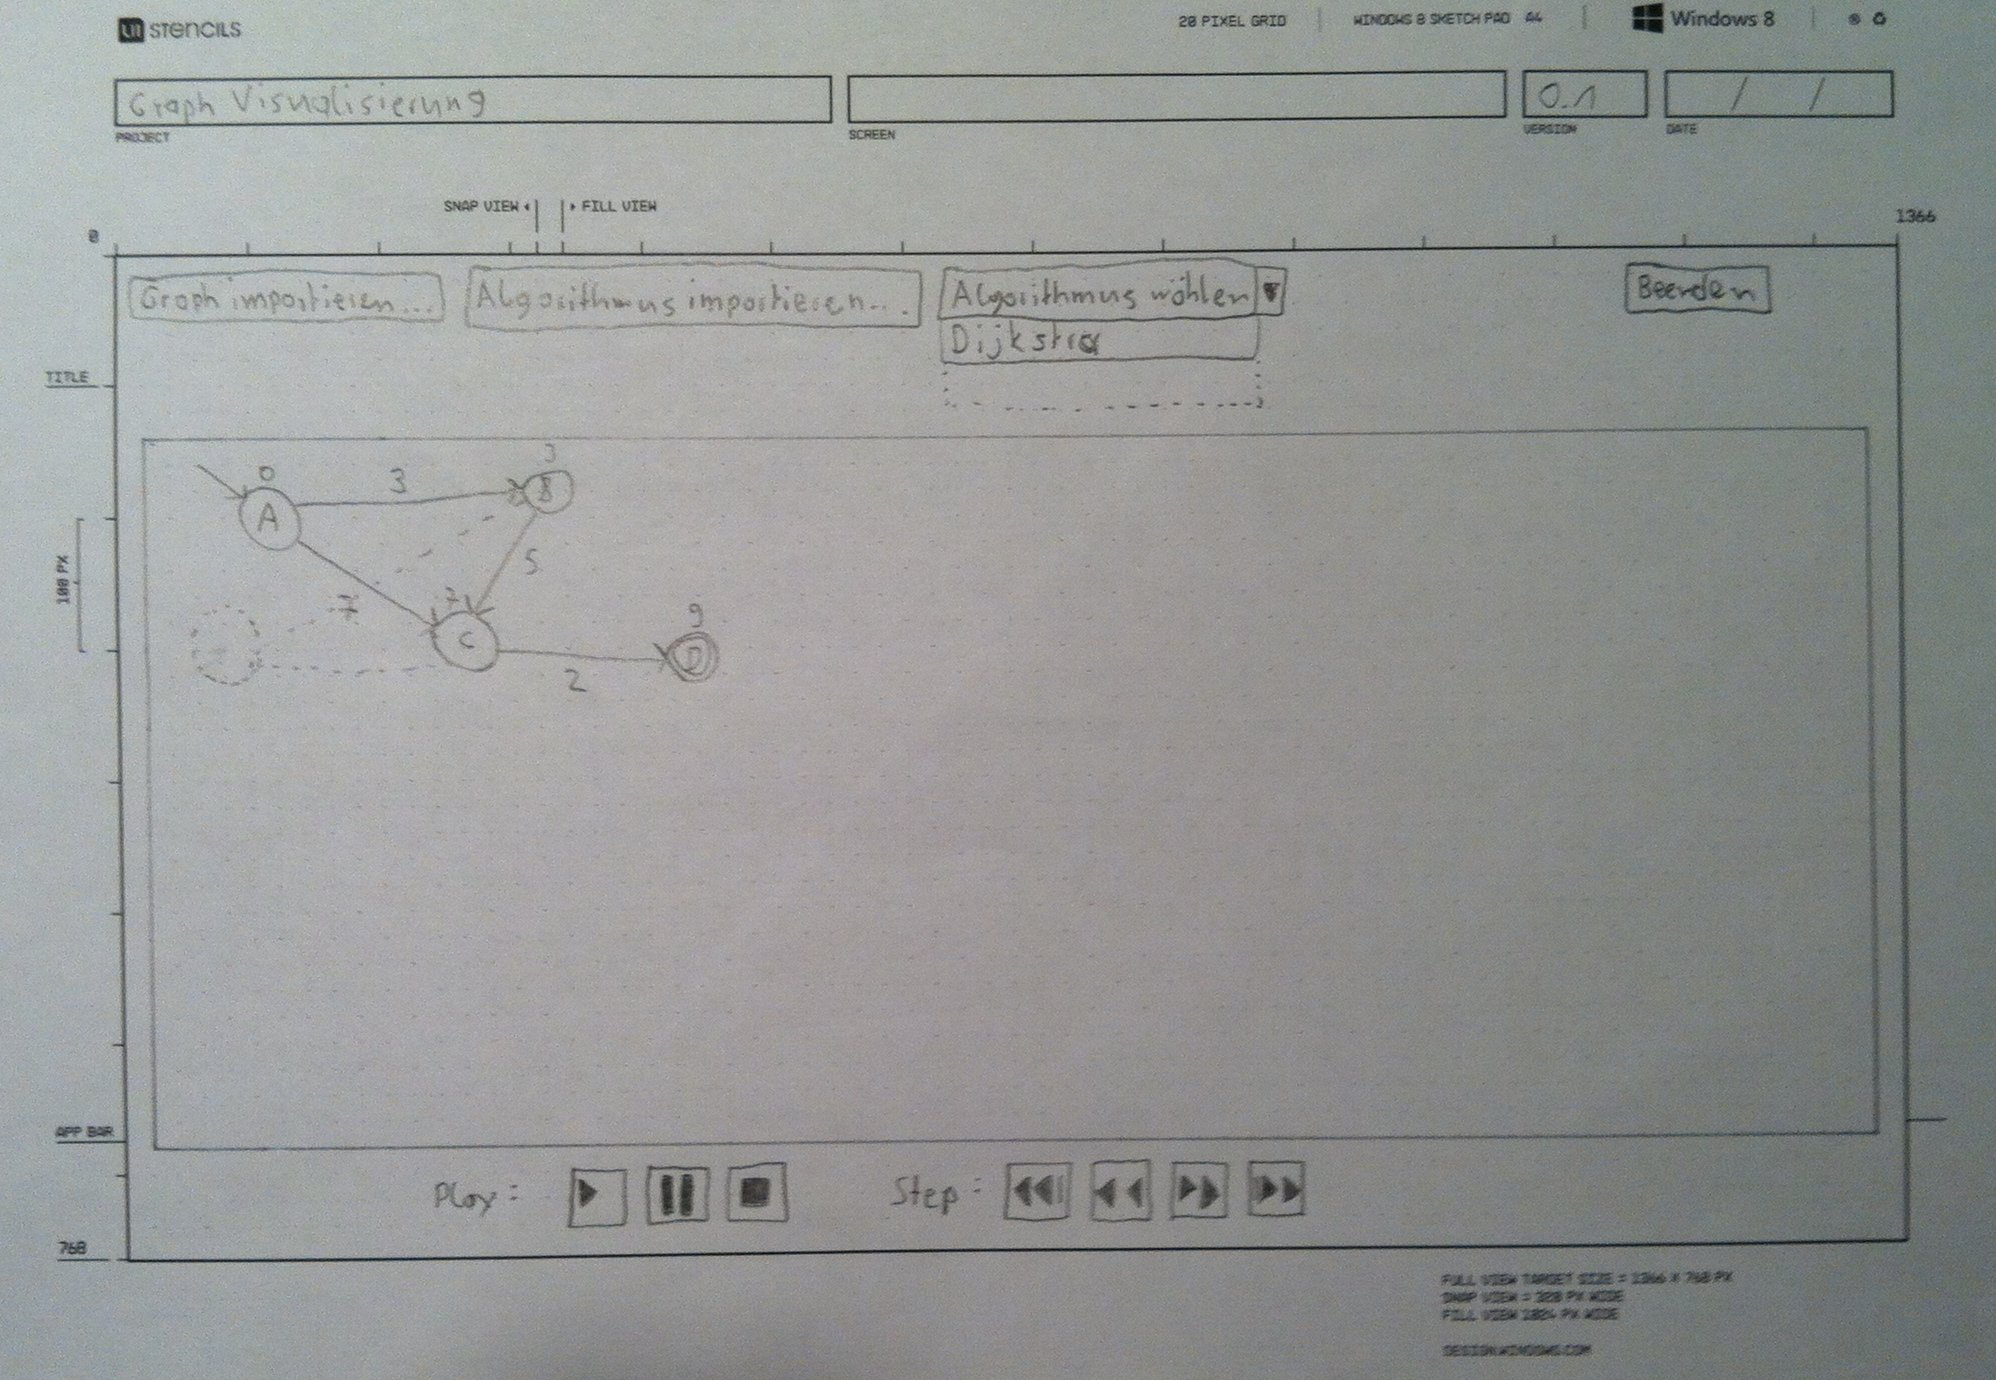
\includegraphics[
% 		    width=\textwidth,
% 		    height=\textheight,
% 		    angle=90,
		    scale=0.1,
		    keepaspectratio=true
    ]{diagrams/architecture/Screen_Sketch_PK_V1_cropped.jpeg}
    \caption{Gui, View: Screen Sketch}
    \label{fig:gui-view-screen-sketch}
\end{figure}
% 
% \section{Data Model}
% \label{sec:Data Model}